\documentclass{article}
\usepackage[utf8]{inputenc}
\usepackage{hyperref}
\usepackage{graphicx}
\usepackage{subfig}

\title{COMP140 Report}
\author{Christopher Robertson}
\date{March 2020}

\begin{document}

\maketitle
\begin{center}
    \href{https://github.com/Koltonix/comp140-arduino-controller}{GitHub}
\end{center}
\newpage

\section{Project Proposal}

The idea for the game is where you control two rotary encoders which will change their LED colour depending on the rotation position. From there you are able to submit the current colour selected on the rotary encoder which will depend on the next colour in the lane. The lane is made from an RGB LED strip which represents the colour queue and the following colours which you must submit in the correct order. If successful you gain a point, but if you do not then you lose the game. As time goes on the speed of the game will increase and therefore become more challenging. I intend for this controller to not depend on Unity, but instead use it as an extended feature. As a result I am primarily programming in C/C++.

\section{Hardware and Components}

There are two main components that I am using for this controller which is the Rotary Encoder (with an LED Light) which acts as the input and output. I also am using an RGB LED strip which only acts as the output for the player and is the primary visuals for the game experience. The other components I'll be using include the Arduino Uno board which will be processing everything and holding the sketch itself. I will also be using a breadboard too as the Arduino Uno doesn't have enough live and ground slots for me to use.

\subsection{Rotary Encoder and RGB LEDs}

\begin{figure}[ht]%
    \centering
    \subfloat[Rotary Encoder]{{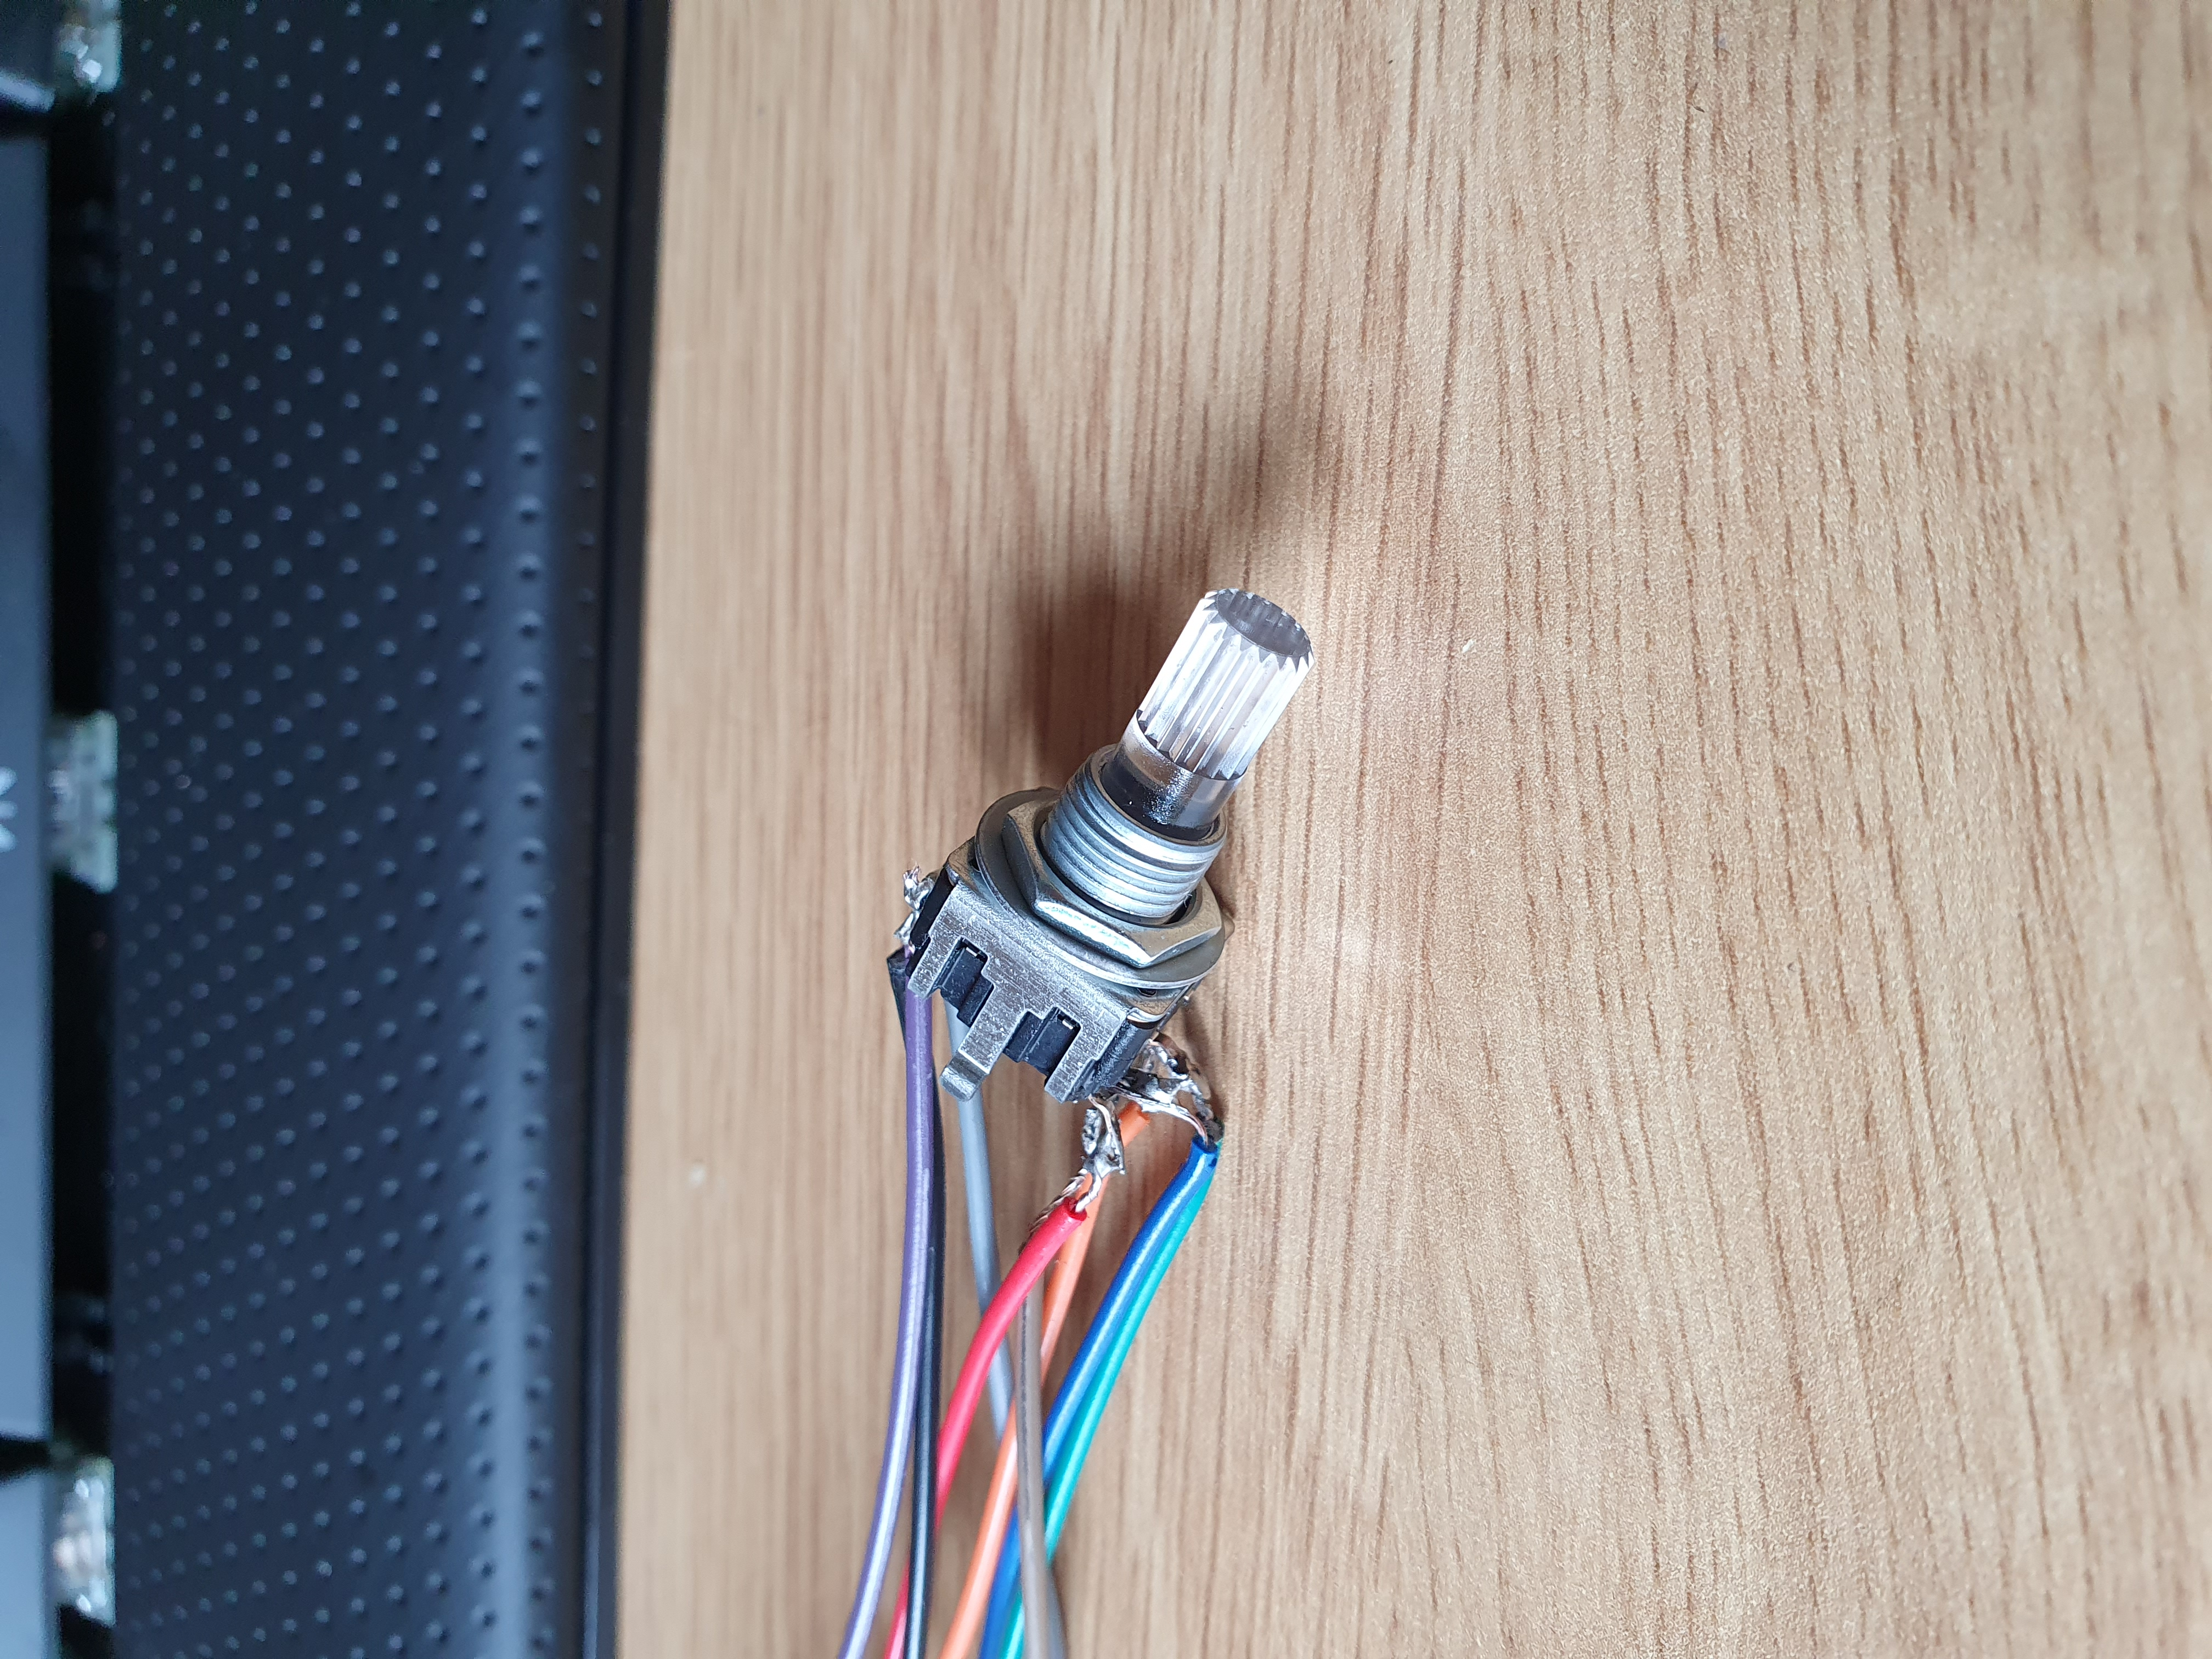
\includegraphics[angle=-90, width=5cm]{rotary_encoder.jpg}}}%
    \qquad
    \subfloat[LED Strip]{{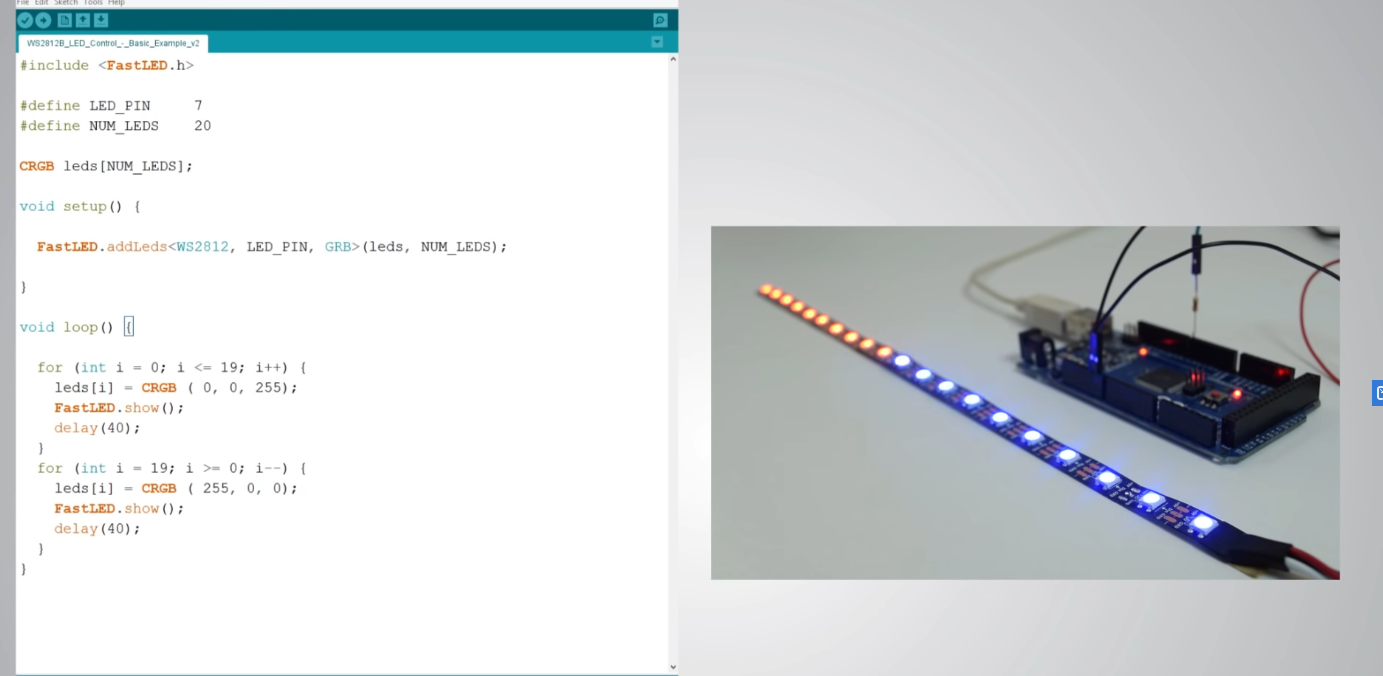
\includegraphics[angle=-90, width=5cm]{led_strip.jpg}}}%
    \caption{External Components}%
    \label{fig:external_component}%
\end{figure}

The rotary encoder is used to control the colour currently selected by rotating the dial which then cycles through an array of available colours. The player is informed of the colour selected by the RGB LED on the rotary encoder itself. Once the player thinks the selected colour is the same as the next colour they press the button to submit. The rotary encoder I have has 8 connections in total; 3 for the RGB, 2 for live and ground, and then 3 for the rotaryA, rotaryB and the button.
\\
\\
The LED RGB Strip is used to feedback the current state of the game to the player. It represents the queue of colours that are next in order. The player will then use the rotary encoder to match the next colour. This piece of hardware only has three connections which are the live, ground and information wire. I am then using the Adafruit Neopixel library to individually address each LED with a different colour.

\subsection{Arduino and Breadboard}

\begin{figure}[ht]%
    \centering
    \subfloat[Arduino Uno]{{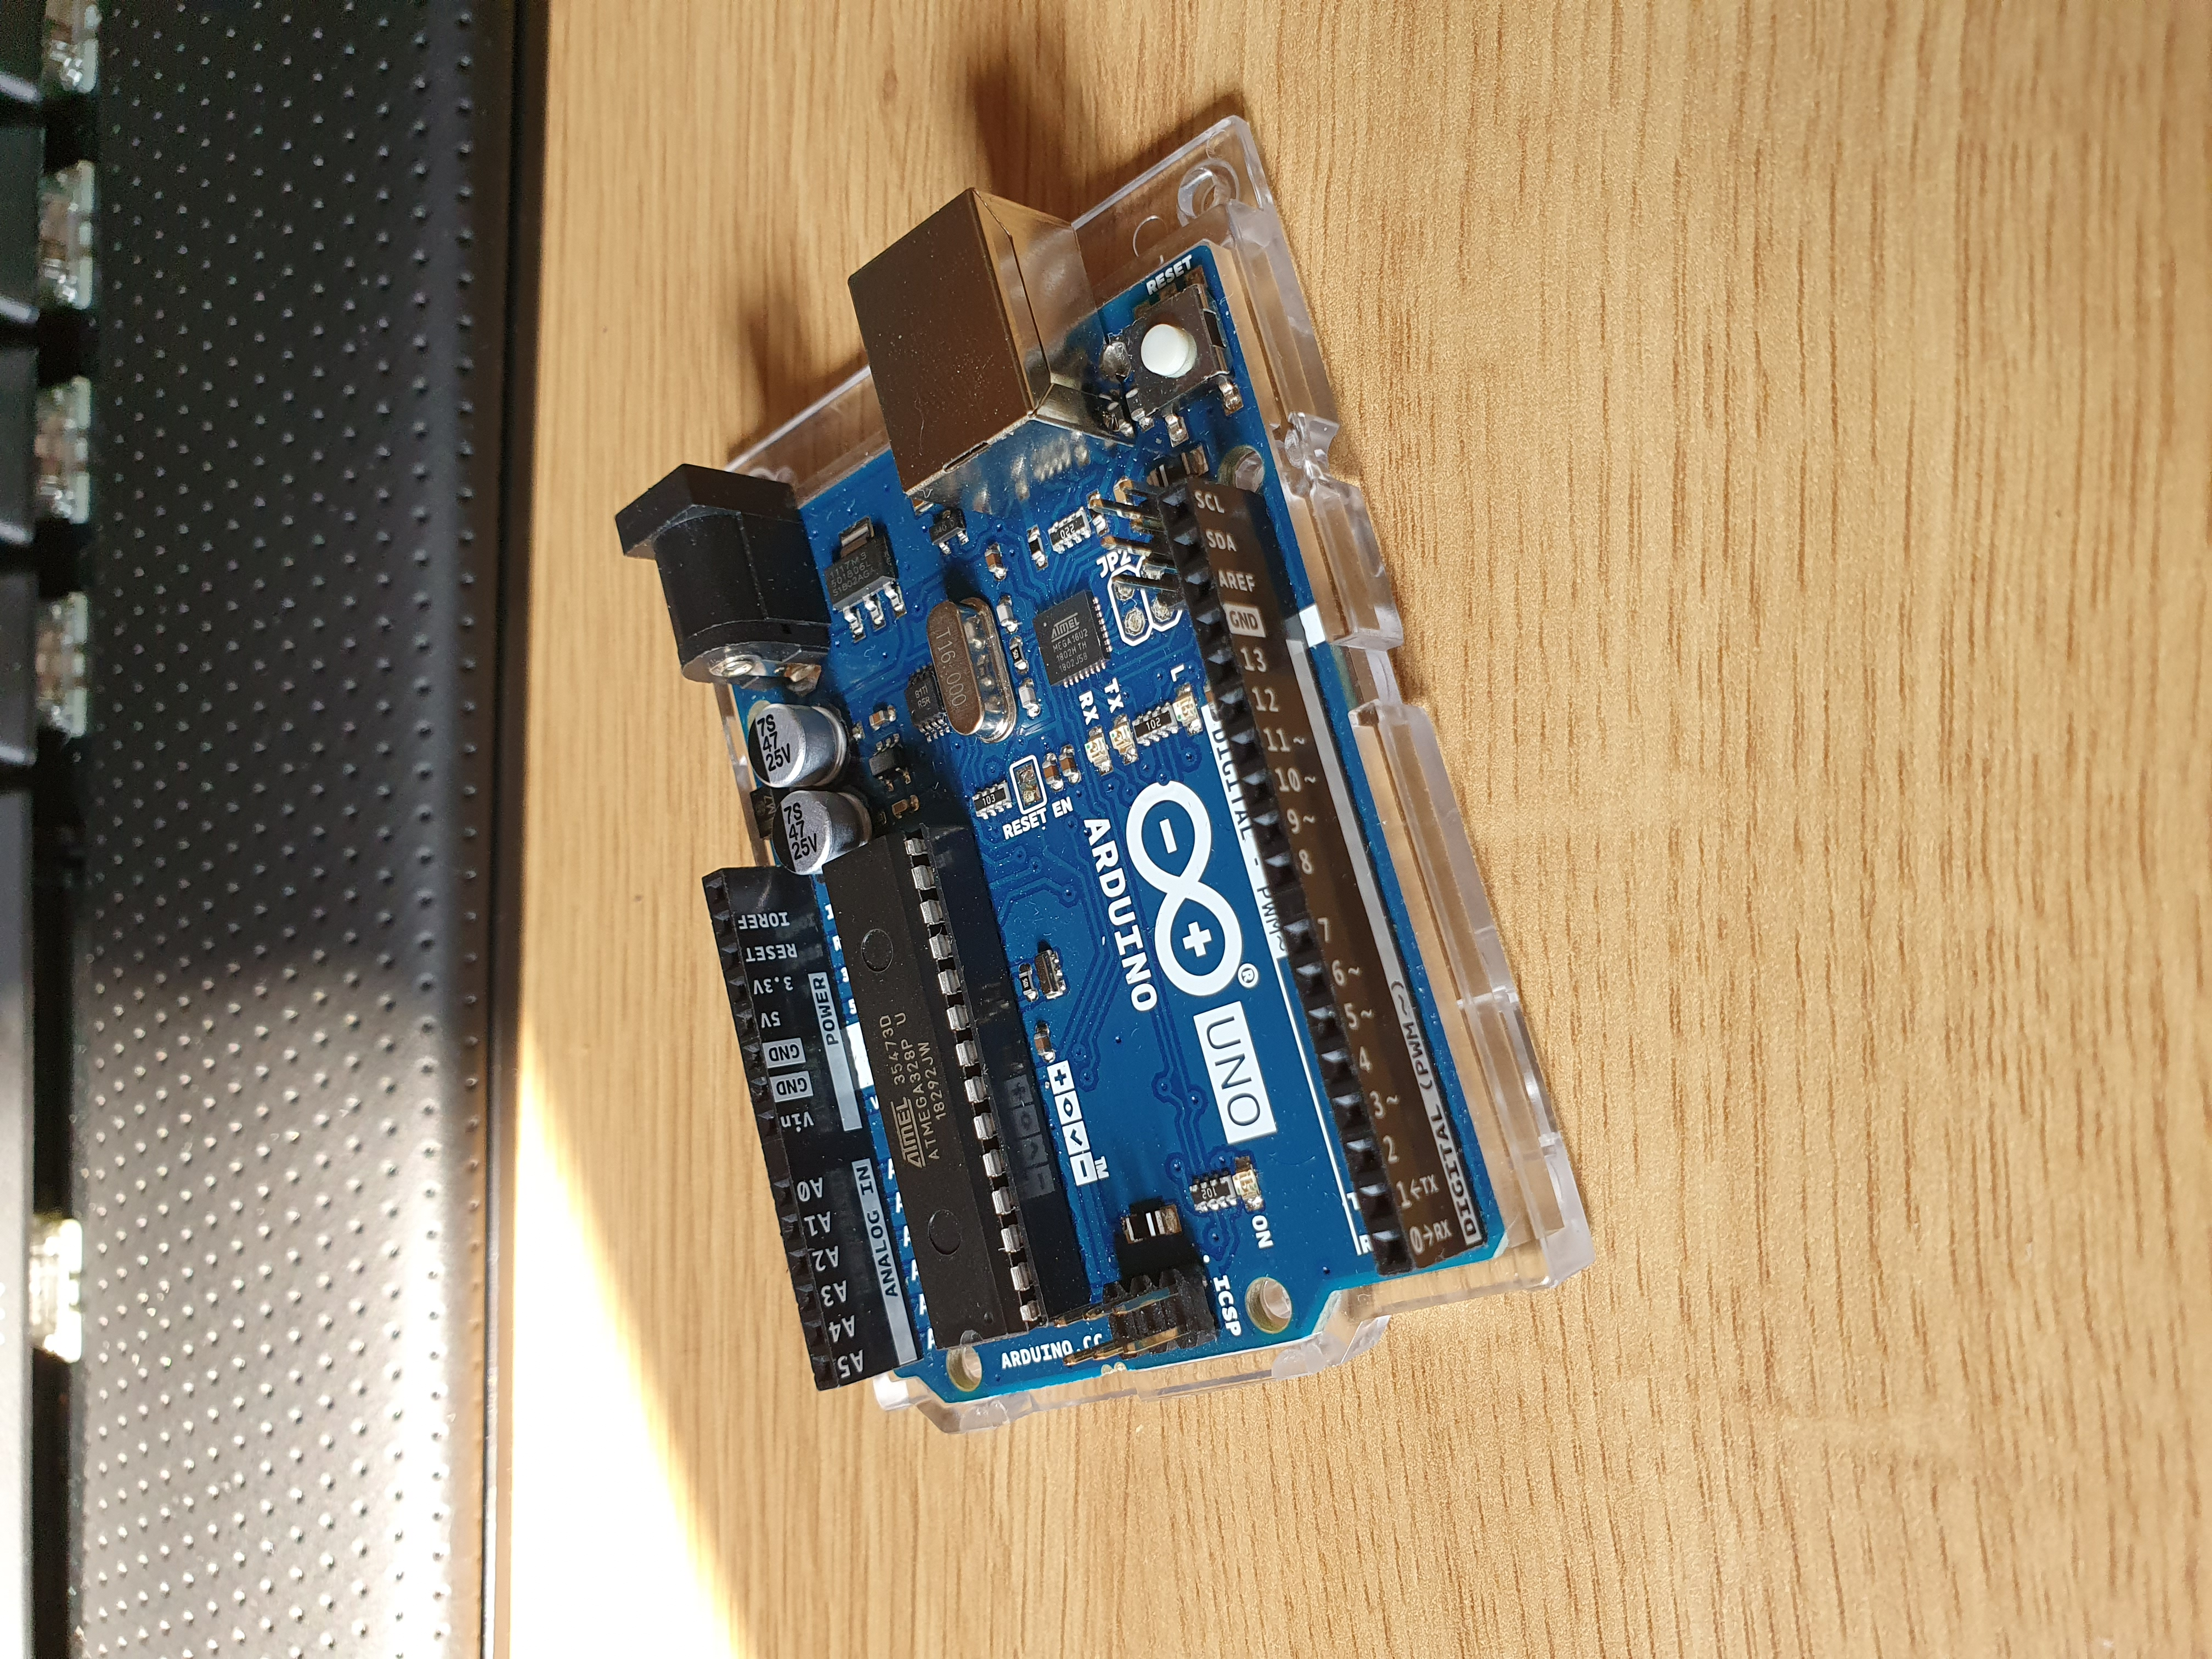
\includegraphics[angle=-90, width=5cm]{arduino-uno.jpg}}}%
    \qquad
    \subfloat[Breadboard]{{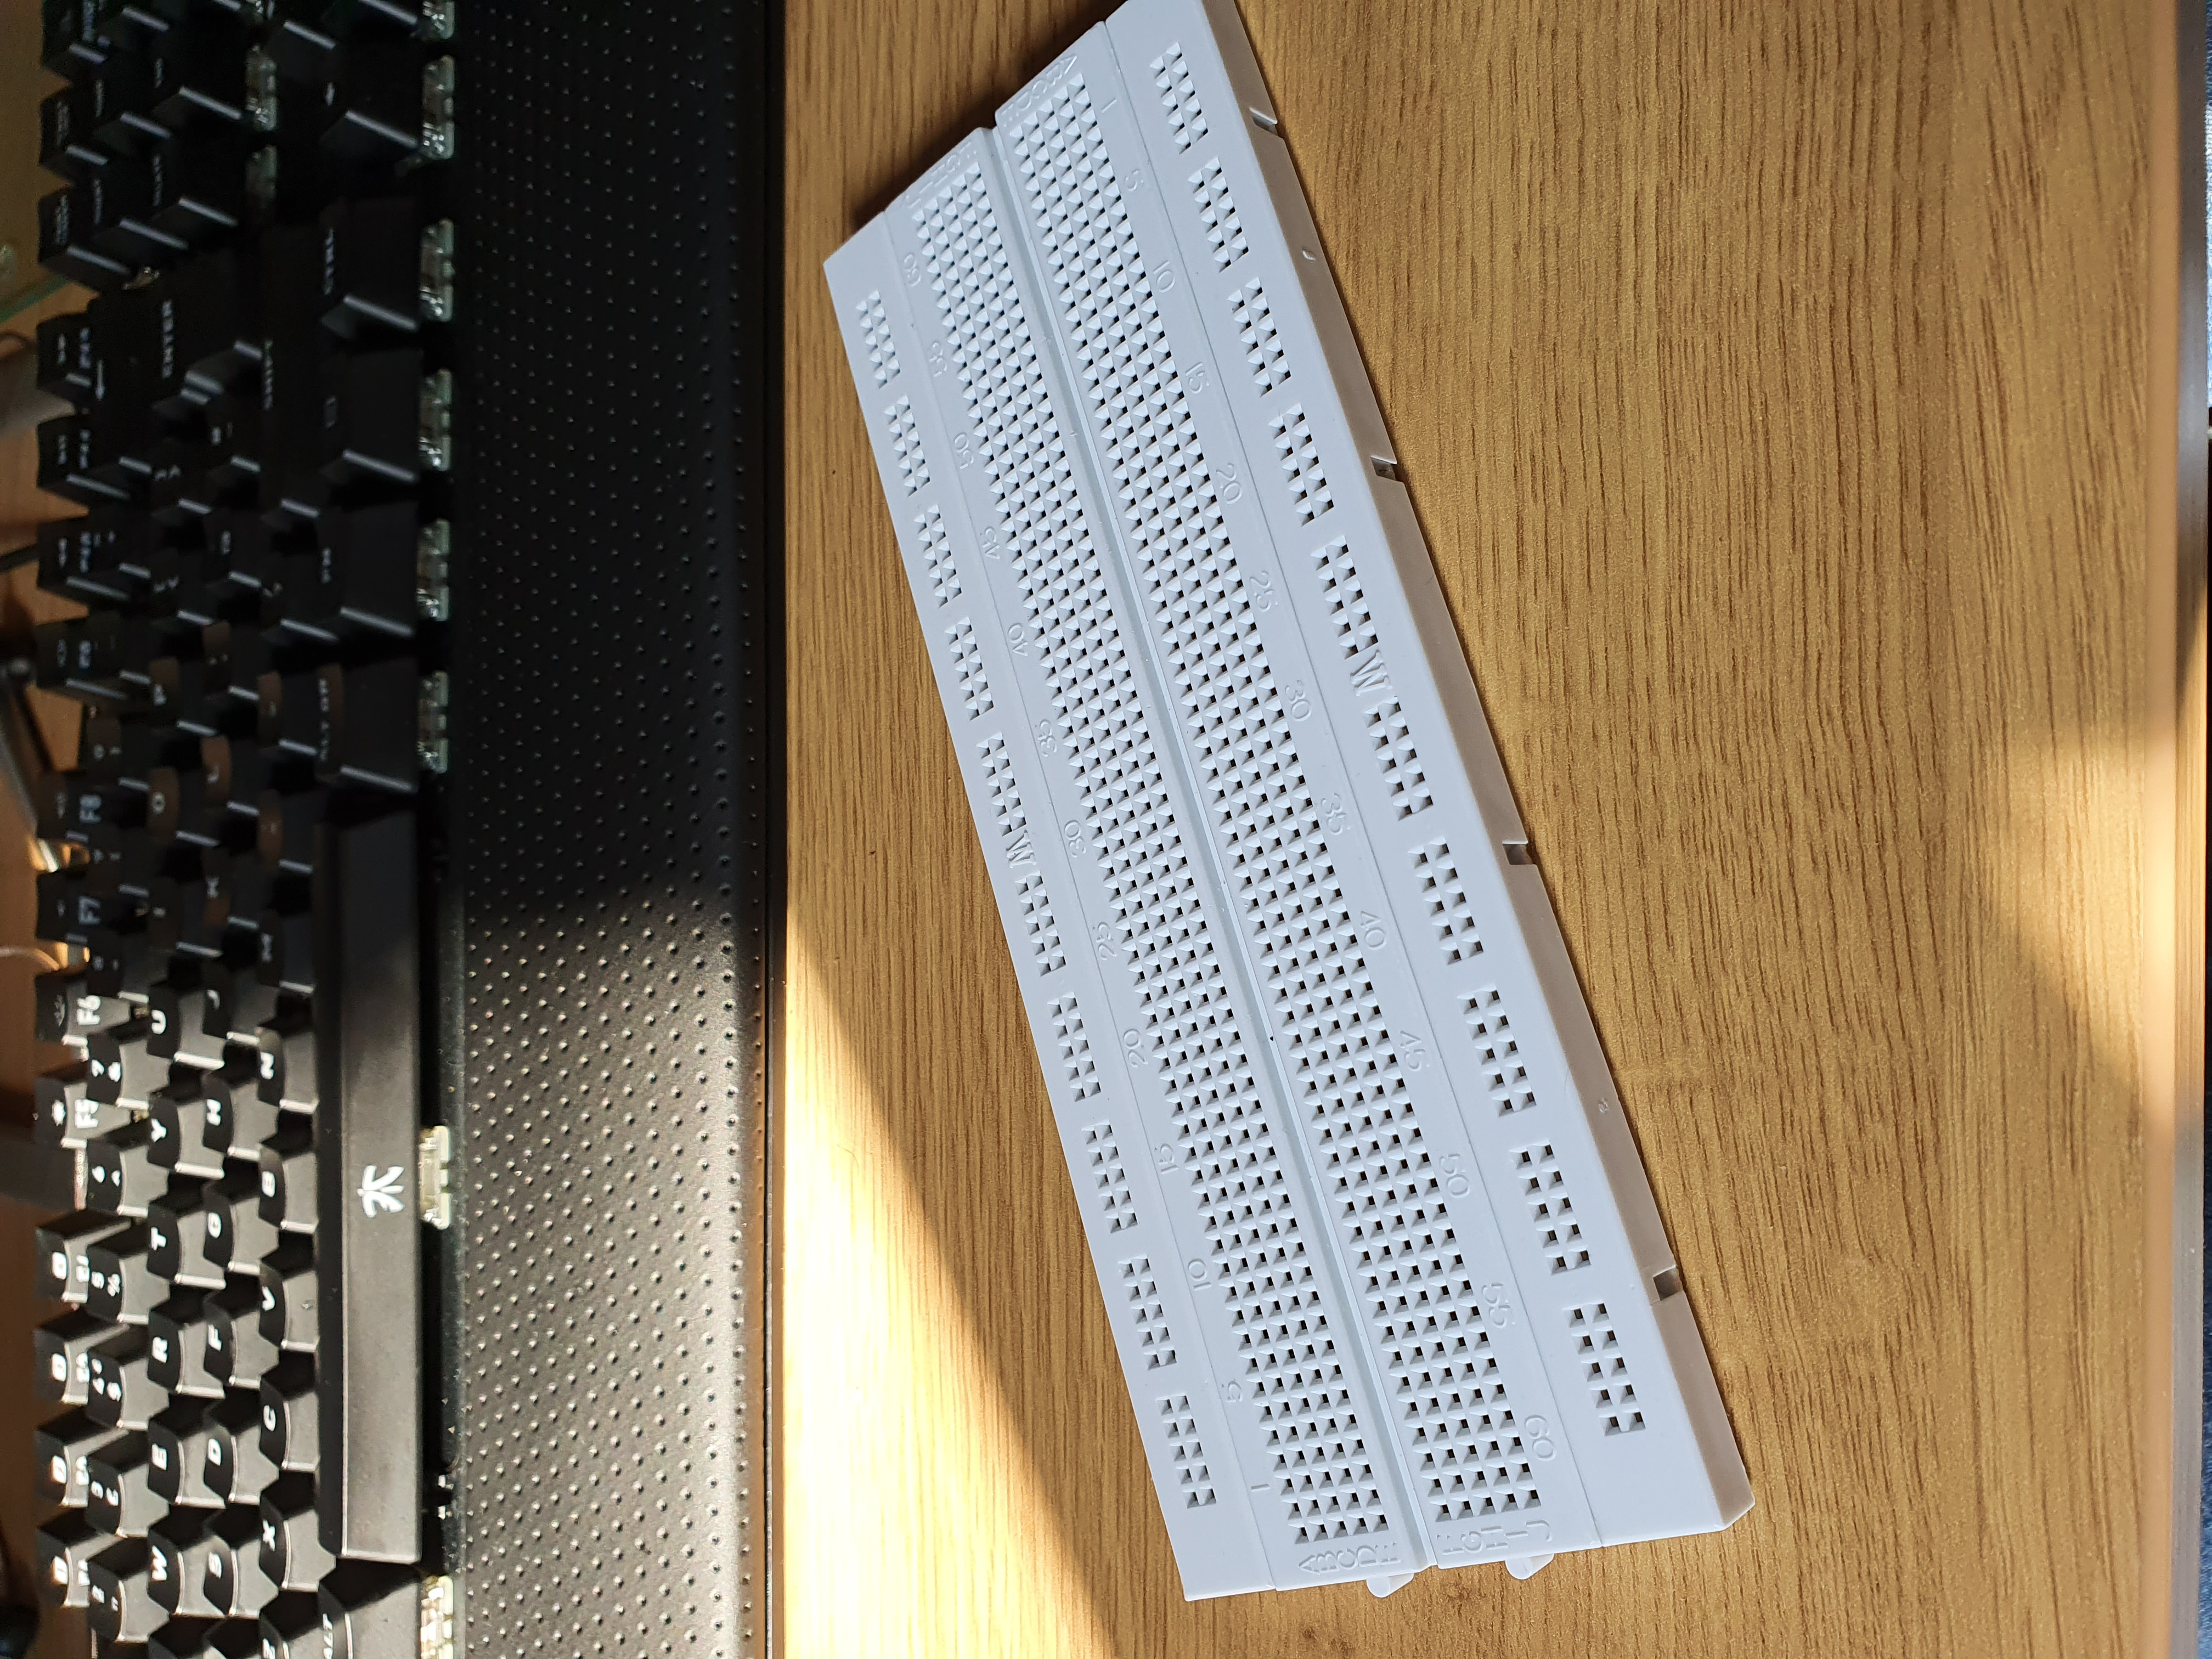
\includegraphics[angle=-90, width=5cm]{breadboard.jpg}}}%
    \caption{Main Hardware}%
    \label{fig:main_hardware}%
\end{figure}

The Arduino will be the main piece of hardware in this project since it will be storing the entire game and the logic behind it. It will take in the input from the rotary encoder and then produce an output to both the rotary encoder LED and the LED strip. This will make the controller entirely in-built and will not require a PC, or more specifically Unity, to run, but will just have Unity as an added debug screen. I will also be using a breadboard as I wouldn't have needed one if the Arduino had 3 extra 5v slots and 1 extra ground slot.

\section{Design of the Controller - Wiring, Casing and Attachments}
\subsection{Design}

\begin{figure}[ht]%
    \centering
    \subfloat[Concept]{{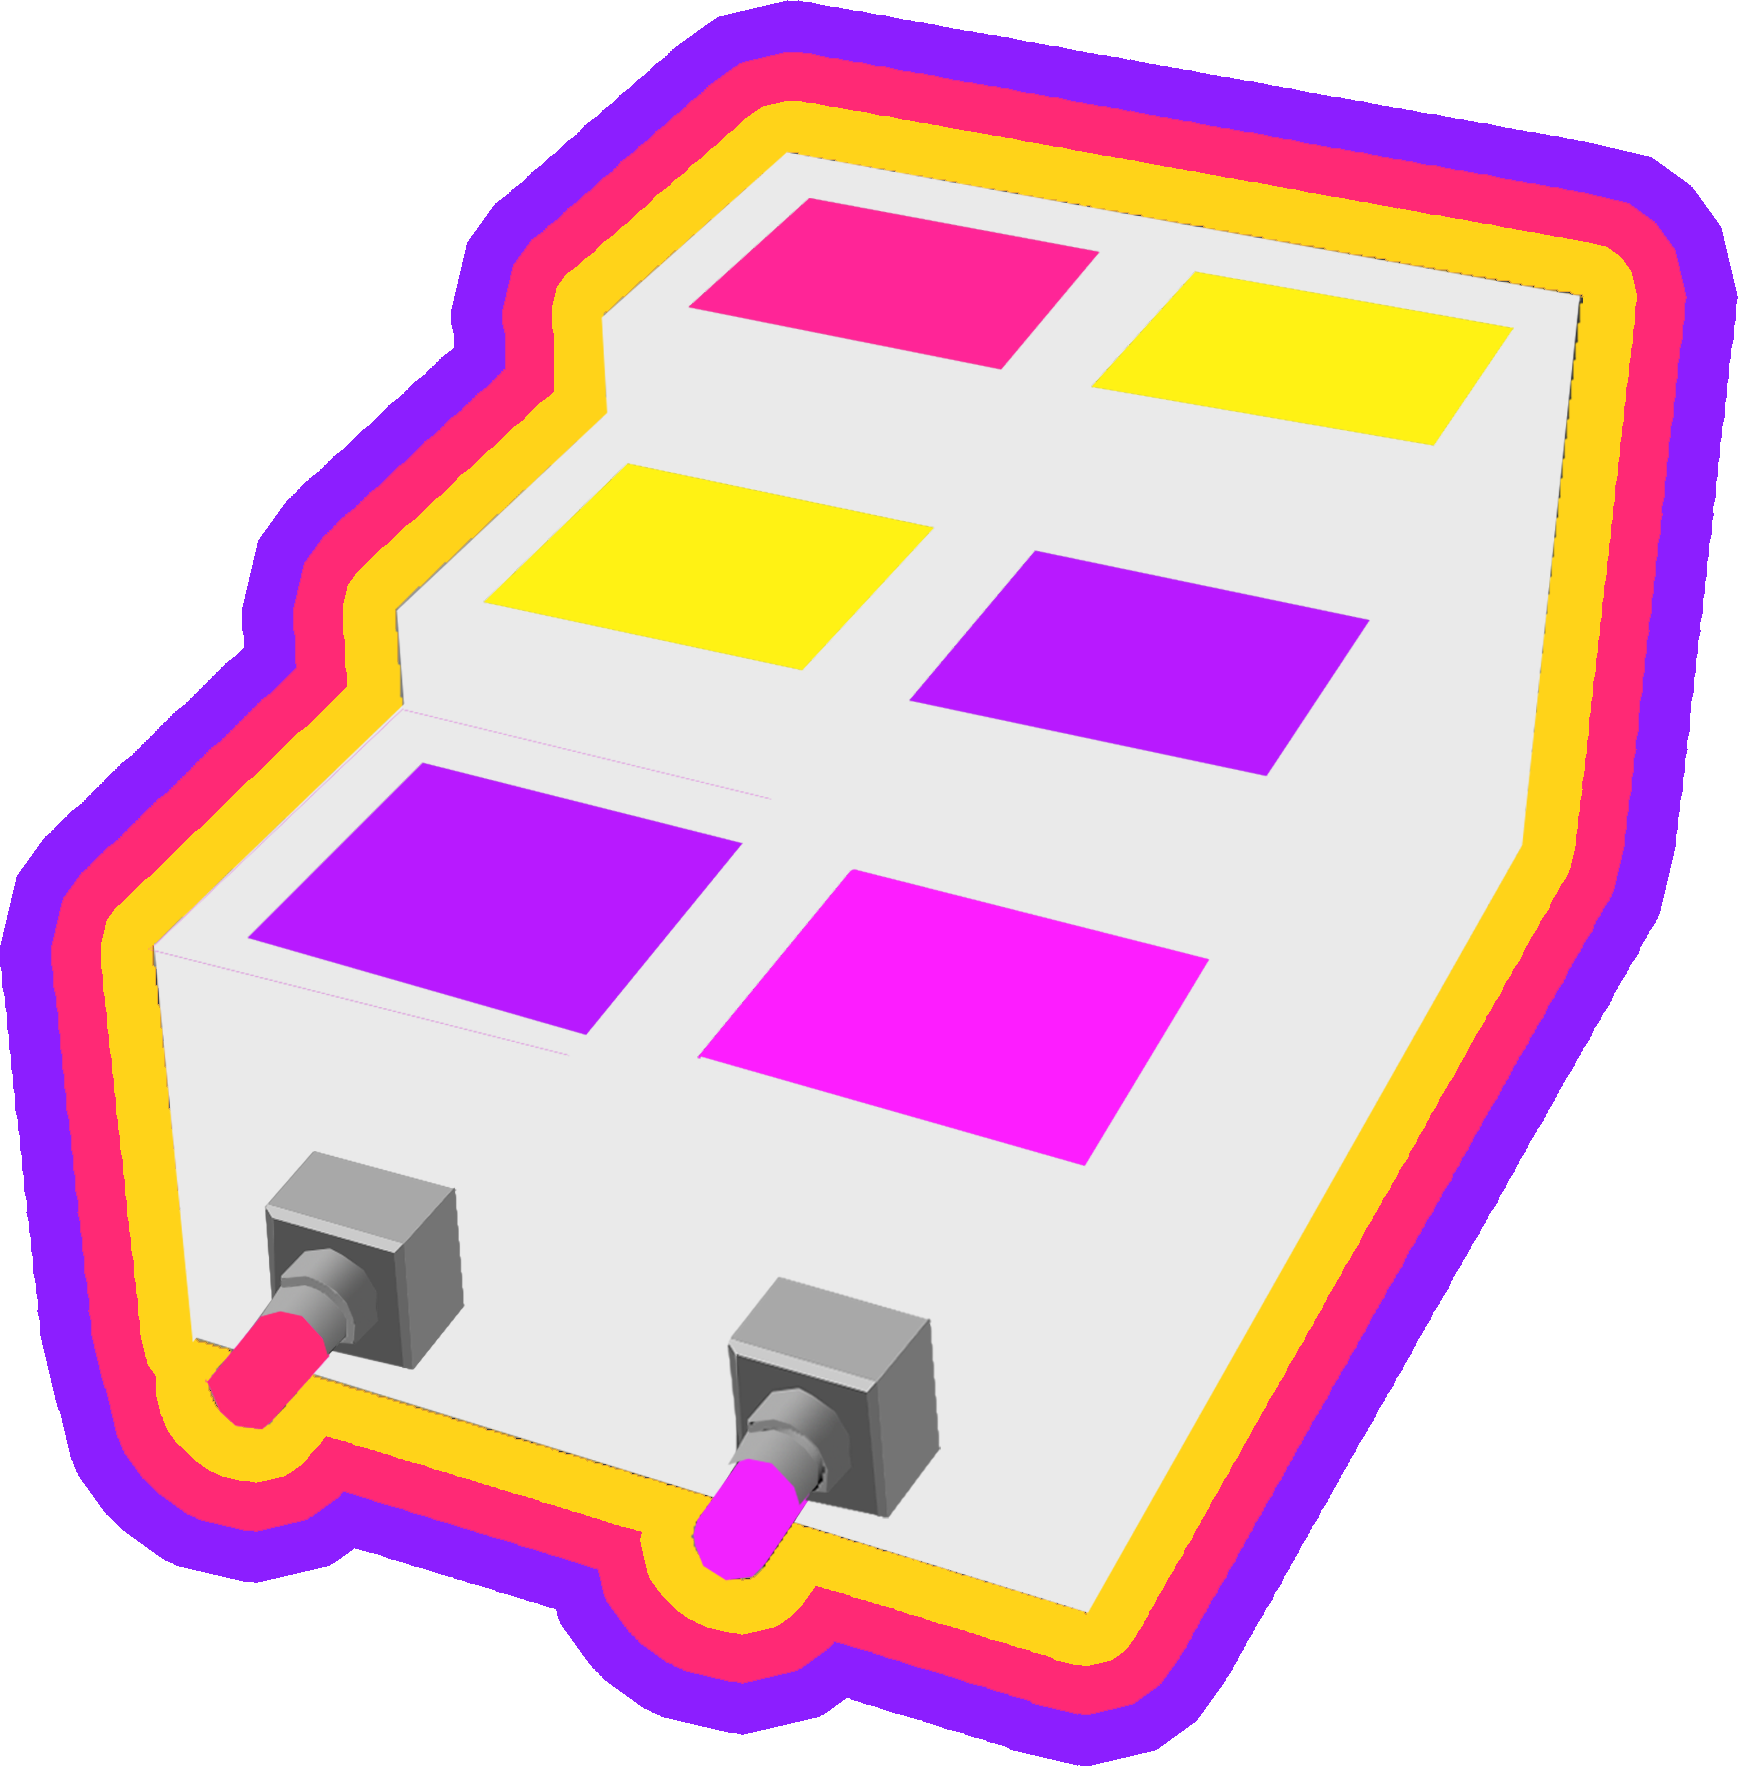
\includegraphics[width=5cm]{controller-concept.png}}}%
    \qquad
    \subfloat[Final]{{\includegraphics[width=5cm]{arduino.png}}}%
    \qquad
    \subfloat[Wiring]{{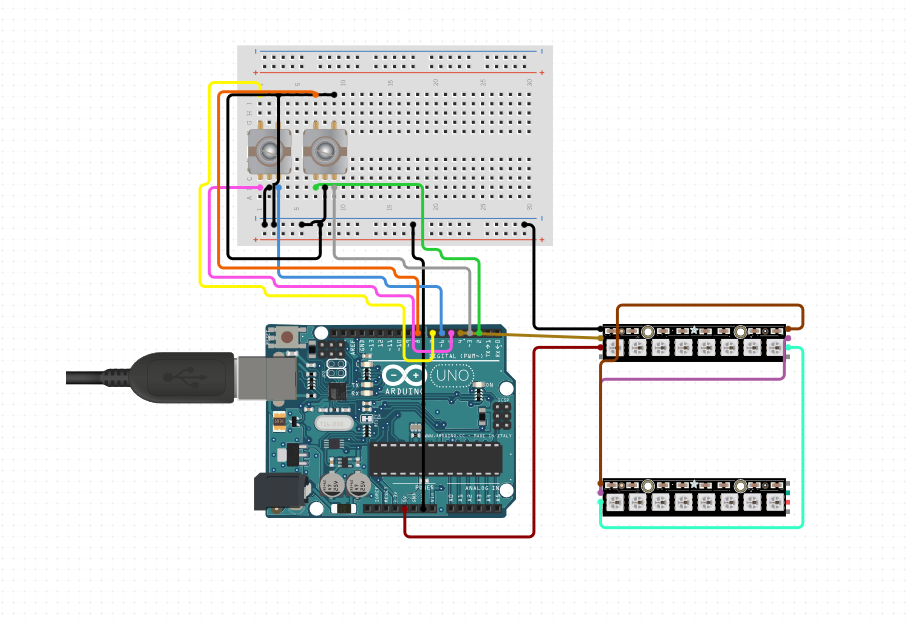
\includegraphics[width=5cm]{arduino-wiring.PNG}}}%
    \caption{Controller Design}%
    \label{fig:controller-design}%
\end{figure}

The design of my controller is to have 3 layers of boxes at 3 separate heights because I feel it is just a bit more aesthetically appealing than just being flat. The top of each of these boxes has a clear layer of plastic so that the player may see the LED colour inside. On the front are the two rotary encoders which are used to control each respective lane. I went for a simple design approach for this and tried to make it look like a sort of toy since that is the kind of game I was making with the in-built controller idea.
\\
\\
The casing of my controller is made out of thick cardboard - although plastic had been planned - where I made 3 sets of rectangular boxes with no top by cutting a sheet of cardboard and using PVA and craft glue to stick it together. Once it had dried I cut around the rough edges and then made each rectangular box its own height in descending order. I then cut the LED strip and wiring holes as well as the slots for the rotary encoder. From there I glued the 3 boxes together to create my final design. I then added some plastic to the top of each box as a lid. The wiring is ran through the controller round to the back where the breadboard and Arduino Uno is stored.
\\
\\
The wiring itself is fairly straight forward. The power and live of the rotary encoders and LED strips are all connected together on the breadboard which is then connected to the Arduino. For the LED strips I then connect the information wire to the breadboard through a resistor and then to its designated digital read slot. This is to prevent it from melting the LEDs. The rotary encoder has all of the remaining wires - RGB and input - wired straight to the Arduino. These can be seen on the diagram.

\section{Game Experience/Concept}
\begin{figure}[ht]
  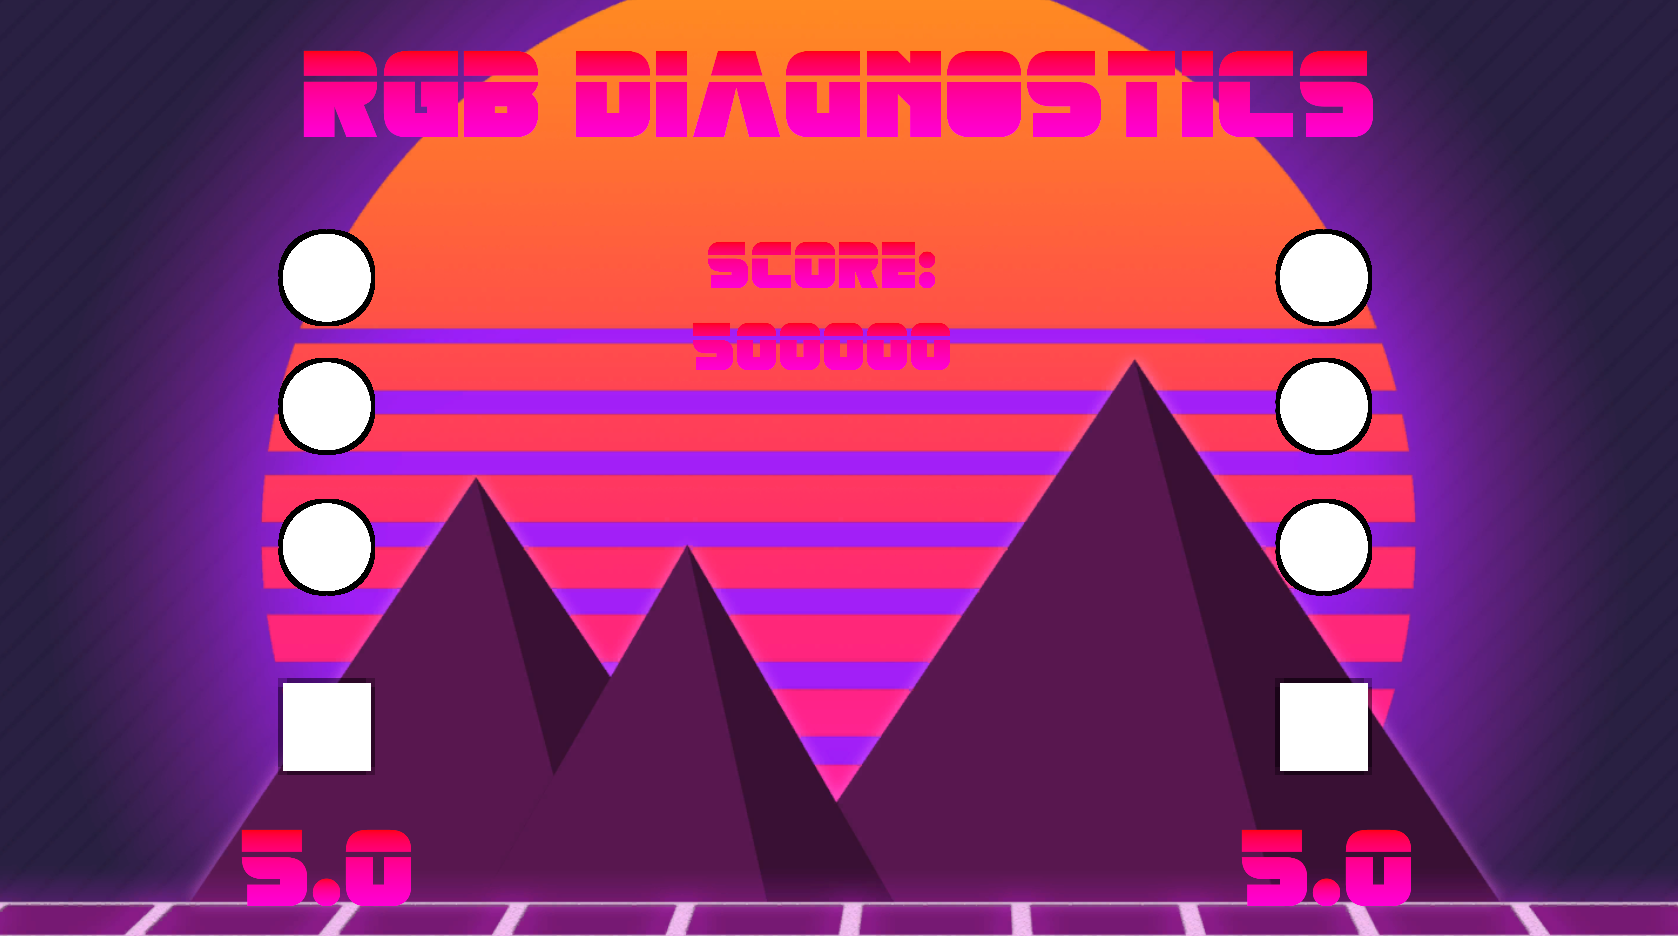
\includegraphics[width=\textwidth,height=\textheight,keepaspectratio]{unity-diagnostics.PNG}
  \caption{Unity Scene}
  \label{fig:unity-diagnostics}
\end{figure}

The game itself is to use the dials to change the colour of the selected colour to match the next one in the queue and will repeat indefinitely much like any sort of arcade game and as time goes on you'll have less time to react. Although the controller will function by itself I also have a debugging game using Unity which allows you to see all of the values on the controller as well as the score since I didn't have enough space on the Arduino for the LCD screen.

\section{Software Design with UML Diagrams}

\begin{figure}[ht]%
    \centering
    \subfloat[Class Diagram]{{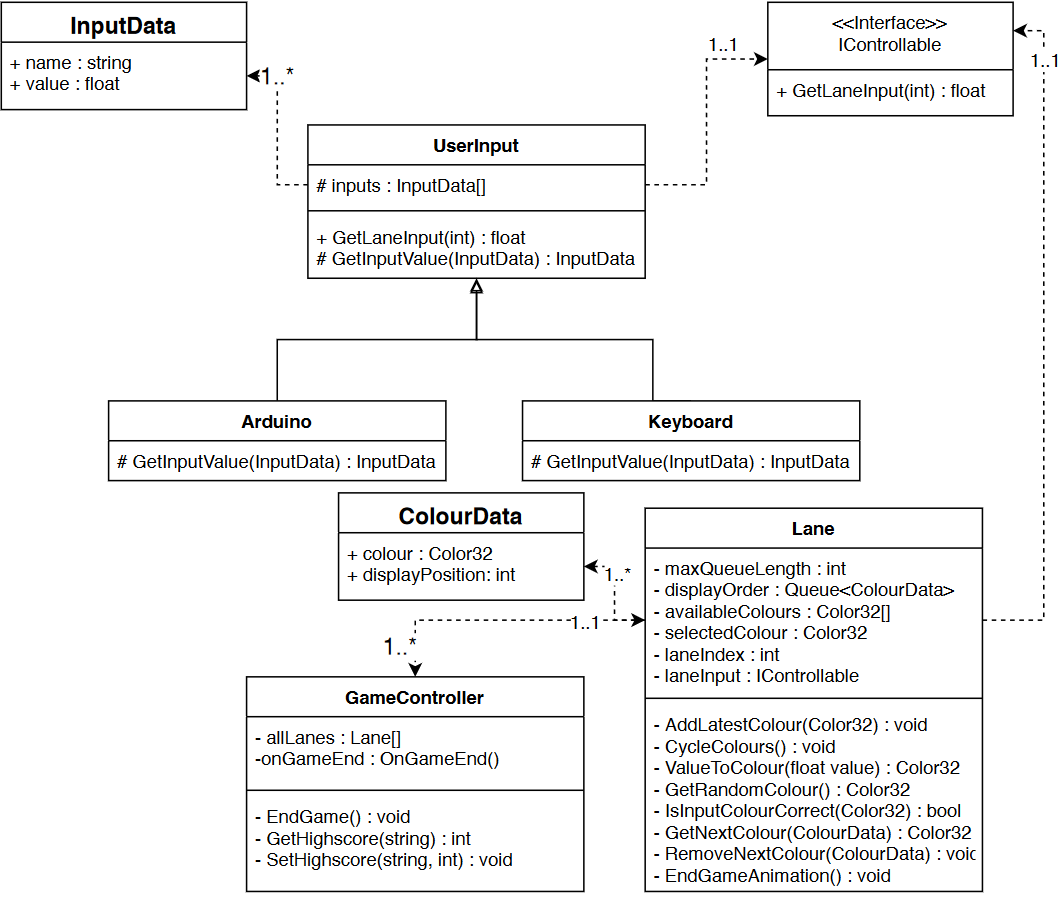
\includegraphics[width=5cm]{uml-class-diagram.PNG}}}%
    \qquad
    \subfloat[Sequence Diagram]{{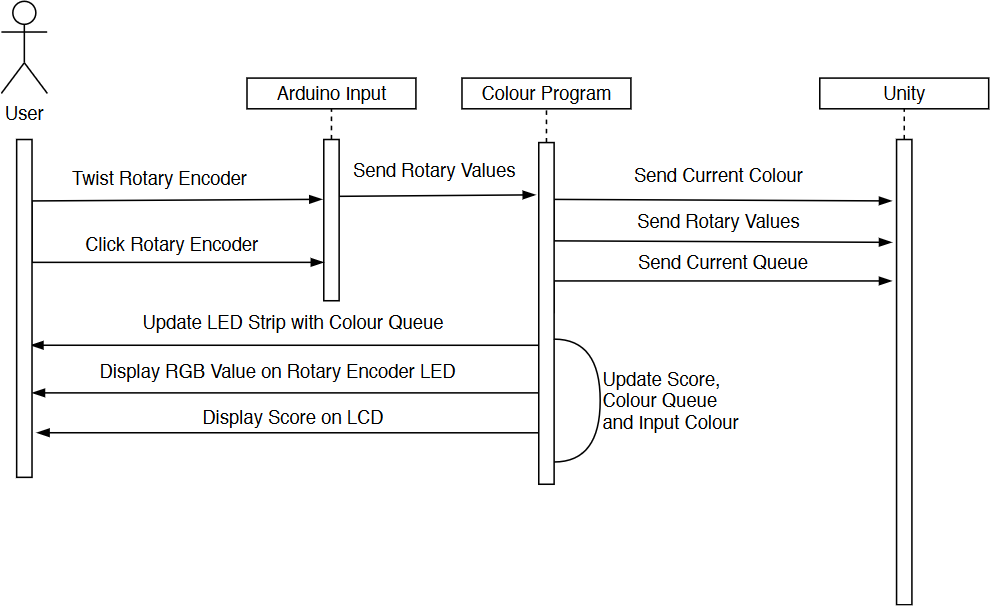
\includegraphics[width=5cm]{uml-sequence-diagram.PNG}}}%
    \qquad
    \subfloat[Case Diagram] {{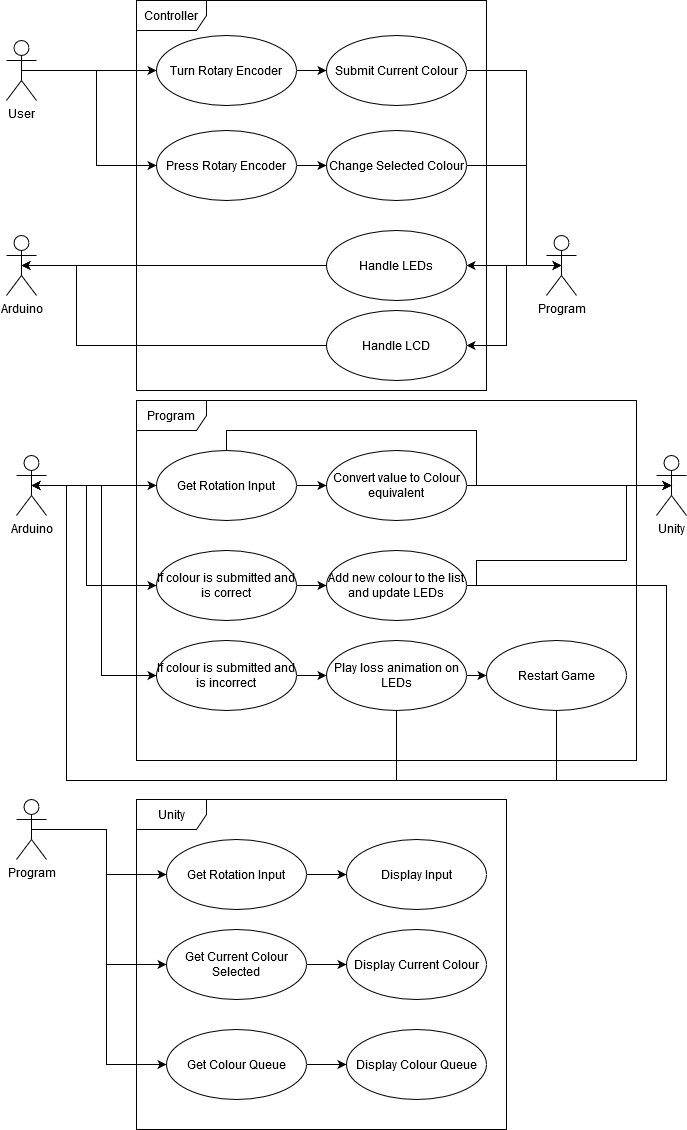
\includegraphics[width=5cm]{uml-case-diagram.png}}}%
    \caption{UML Diagrams}%
    \label{fig:uml-diagrams}%
\end{figure}

\subsection{Arduino Ports}
In hindsight, one area would have benefit me from the would have been to look into how many ports all of my components would need since I only realised once I had the physical components that I would have too few slots for everything I needed hence the scaling back in the size of my controller and the features.
\\

\subsection{Rotary Encoders}
Once again, it would have been to my benefit to look more into the research of how to hook up the rotary encoder that I bought rather than assuming other encoders would work in the exact same way since the main issue that I had with my rotary encoder was the lack of resources on what each connection was and I had only found out through one forum post; however, in terms of the firmware itself the rotary encoder went quite smoothly compared to what I had first imagined as it is only a short and simple function to get the data into a readable format.
\\

\subsection{Soldering}
Another difficult area was the soldering since I had never actually done it before, but did watch a couple of videos on how to do it. Overall, I was successful in soldering; however, I didn't do the best job of it mainly due to a lack of holding equipment for the components, so in the future I'd look into buying a clamp/stand to make my life infinitely easier when soldering.
\\

\subsection{C++ in General}
Since my controller is entirely independent from any other system except the Arduino I needed to code everything in C++ which proved to be quite a challenge mainly due to the debugging difficulties. One example is where I spent a fair amount of hours trying to figure out a pointer issue that I was having and finally narrowed it down to an array that wouldn't work one tenth of the time; however, this project has been exceptional practice for C++.
\\

\subsection{C++ Arduino Libraries}
A final issue I had near the deadline was that the libraries that I had used when testing the C++ code in a separate environment. The issue with the libraries was that the Arduino didn't support them which was a problem since I relied on the queues and vectors in the their respective library, but luckily there were a variety of custom libraries that I could use to replace instead.
\\

\subsection{Summary}
Looking back at this project I'm quite pleased overall with the final product I have produced in regards to what I had intended from my proposal since although I did have to cut back the LCD screen and three lane idea I have still been able to produce the in built controller that I've wanted to make from the start using LEDs and a rotary encoder.
\end{document}
